\subsection{Design of the dataflow}\label{subsec:dataflow}

\textbf{work in progress}

Gathering and structuring the data is quite a nuisance in a project like ours. The stores and retailers do not put official prices of everything, they only issue a catalog with the offers they have, once a month. The figure \figref{fig:dataflow} shows the absolute overall design of the dataflow, and it illustrates the trouble of gathering information. The recipes have to be gathered from a free website or from the users using the application, however we need some sort of base of recipes for people to actually use the application in the first place. Opskrifter.dk is a huge online database with around 3.000 different recipes, and these are the recipes we intend to use and work with in our application. This part seems rather trivial, however adjusting recipes for spell errors and matching them with the right ingredients can be problem, and requires some string analysis and management. It will be possible for us as the developers to control the data, and a lot of the work have to be done manually, as it is extremely hard to catch all of the problems with the recipes.

The Ingredient data is, as mentioned, something entirely more complicated. We made an agreement with Statistics Denmark for the average prices of groceries across stores and retailers and planned to use these as a base for all calculations. All of this data is functioning as a good base, it does however not portray a completely true image of each store and retailer. It will resolve in some values as to savings and price, that wont be 100\% correct -which is why our application only can be seen as a guidance and estimate of the price and savings. The offers for the different groceries are gathered through eTilbudsAvisen. It is an online service which gathers all offers offered by a selection of retailers in Denmark, and it does so by traversing the catalogs and extracting all the data. They offer all their data through a web Api, and the idea is for us to download their entire database once a day, and make the calculations necessary for it to match our database. 

\begin{figure}
\label{fig:dataflow}
\centering
\includegraphics[width=0.95\textwidth]{Pictures/dataflow}
\caption{A model of the dataflow through the entire system}
\end{figure}

\paragraph{Design of the Database}
\label{para:dbdesign}

The database is major part of the server, and a big part of the application is dependent upon the database being frequently and correctly updated. Furthermore the database has to be designed in a way that makes calculations fast to access and compute, as we do not want the user to wait for long queries and joins in order to get something shown on the application. We have chosen to work with a physical server and abstained from using the cloud because we have huge amount of data, which requires daily updates and further development. Since we do not have problems maintenance or the costs of renting a server, this was by far the most optimal solution.

\begin{figure}
\label{fig:ER-diagram}
\centering
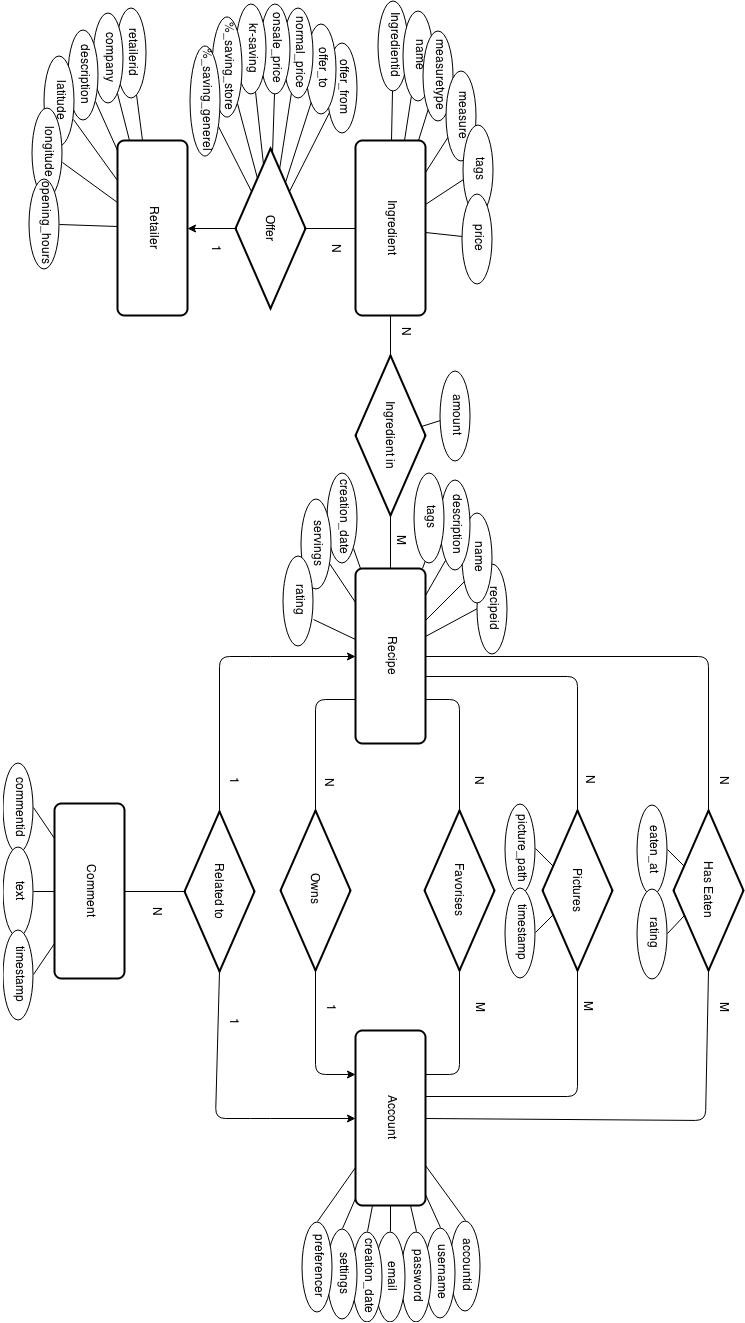
\includegraphics[width=0.95\textwidth]{Pictures/ERdiagram}
\caption{The final ER diagram of the database}
\end{figure}

A lot of these relations speak for themselves, and the entire amount of relationships between account and recipe rather intuitive. We have chosen not to gather all the data in a single relationship as we want perform quick queries on the database rather than save memory. This is one of the advantages of having a stationary server with a large amount of memory available, it is possible to focus solely on performance. 

The biggest table in terms of sheer numbers would be ingredientIn, as each recipe has a lot of different ingredients. This has been accommodated for by moving most attributes to either recipe or ingredient, and we make sure to query through IngredientIn before joining any of these together.

